\documentclass{article}

\usepackage{arxiv}

\usepackage[utf8]{inputenc} % allow utf-8 input
\usepackage[T1]{fontenc}    % use 8-bit T1 fonts
\usepackage{hyperref}       % hyperlinks
\usepackage{url}            % simple URL typesetting
\usepackage{booktabs}       % professional-quality tables
\usepackage{amsfonts}       % blackboard math symbols
\usepackage{nicefrac}       % compact symbols for 1/2, etc.
\usepackage{microtype}      % microtypography
\usepackage{lipsum}
\usepackage{graphicx}
\usepackage{subfigure}
\usepackage{placeins}
\usepackage{enumerate}
\usepackage{amsmath}
\DeclareMathOperator*{\argmin}{arg\,min}
\DeclareMathOperator*{\argmax}{arg\,max}


\title{Entropy-Scaling Hierarchical Compression and Search of Large High-Dimensional Datasets via an Actualization of the Manifold Hypothesis}


\author{
    Najib Ishaq \\
    Department of Computer Science and Statistics\\
    University of Rhode Island \\
    Kingston, RI \\
    \texttt{najib\_ishaq@uri.edu} \\
    \And
    Thomas J. Howard III \\
    Department of Computer Science and Statistics\\
    University of Rhode Island\\
    Kingston, RI\\
    \texttt{thoward27@uri.edu} \\
    \AND
    Noah M. Daniels \\
    Department of Computer Science and Statistics\\
    University of Rhode Island\\
    Kingston, RI\\
    \texttt{noah\_daniels@uri.edu} \\
}

\date{}

\begin{document}

    \maketitle
    \begin{abstract}
        Abstract is written last \dots
    \end{abstract}

    \section{Introduction}
\label{sec:introduction}

Researchers are collecting data at an unprecedented scale.
In many fields, the sizes of datasets are growing exponentially, and this increase in the rate of data collection outpaces improvements in computing performance as predicted by Moore's Law~\cite{kahn2011future}.
This indicates that the performance computer hardware will not ``catch up'' to computational needs in the near future.
Often dubbed ``the Big Data explosion,'' this phenomenon has created a need for better algorithms to analyze large datasets.

Examples of large datasets include genomic databases, time-series data such as radio frequency signals, and neural network embeddings.
Large language models such as GPT~\cite{2020arXiv200514165B, OpenAI2023GPT4TR} and LLAMA-2~\cite{Touvron2023Llama2O}, and image embedding models~\cite{radford2021learning, dosovitskiy2020image} are a common source of neural network embeddings.
These embeddings are often high-dimensional, and the sizes of training and inference datasets for such networks are growing exponentially.
Among biological datasets, the GreenGenes project~\cite{desantis2006greengenes} provides a multiple-sequence alignment of over one million bacterial 16S sequences, each 7,682 characters in length, while SILVA 18S~\cite{10.1093/nar/gks1219} contains ribosomal DNA sequences of approximately 2.25 million genomes with an aligned length of 50,000 letters.
Among time-series datasets, the RadioML dataset~\cite{oshea2018radioml} contains approximately 2.55 million samples of synthetically generated signal captures of different modulation modes over a range of SNR levels.

Many researchers are especially interested in similarity search on these datasets. 
Similarity search enables a variety of applications, including recommendation~\cite{annoy} and classification systems~\cite{suyanto2022knnclassifier}. 
As the cardinalities and dimensionalities of datasets have grown, however, efficient and accurate similarity search has become extremely challenging; 
even state-of-the-art algorithms exhibit a steep tradeoff between recall and throughput~\cite{Malkov2016EfficientAR, johnson2019billion, annoy, aumuller2020ann}.

Given some measure of similarity between data points, e.g. a distance function, there are two common definitions of similarity search: $k$-nearest neighbor search ($k$-NN) and $\rho$-nearest neighbor search ($\rho$-NN).
$k$-NN search aims to find the $k$ most similar points to a query, while $\rho$-NN search aims to find all points within a similarity threshold $\rho$ of a query.

Previous works have used the term \textit{approximate} search to refer to $\rho$-NN search, but in this paper, we reserve the term \textit{approximate} for search algorithms which do not exhibit perfect recall when compared to a na\"{i}ve linear search.
In contrast, an \textit{exact} search algorithm exhibits perfect recall.

$k$-NN search is one of the most ubiquitous classification and recommendation methods in use~\cite{fix1952discriminatory, cover1967nearest}.
Na\"{i}ve implementations of $k$-NN search, whose time complexity is linear in the dataset's cardinality, prove prohibitively slow for large datasets or those whose cardinalities are growing exponentially.
While fast algorithms for $k$-NN search on large datasets exist, most do not exploit the geometric and topological structure inherent in these datasets.
Further, such algorithms are often approximate~\cite{gao2023high}, and while approximate search may be sufficient for some applications, the need for efficient and \textit{exact} search remains~\cite{ukey2023survey}.

For example, for a majority voting classifier, approximate $k$-NN search may agree with exact $k$-NN search for large values of $k$, but may be sensitive to local perturbations for smaller values of $k$.
This is especially true when classes are not well-separated~\cite{zhang2022imbalanced}.
Further, there is evidence that distance functions which do not obey the triangle inequality, such as cosine distance, perform poorly for $k$-NN search in biomedical settings~\cite{hu2016distance};
this suggests that approximate $k$-NN search could exhibit suboptimal classification accuracy in such contexts.

$\rho$-NN search also has a variety of applications.
For example, one could search for all genomes within a maximum edit distance of a query genome to find evolutionarily-related organisms~\cite{budowski2010fragbag}.
One could also search for all words within a maximum edit distance of a misspelled word to suggest corrections~\cite{ukkonen1985algorithms}.
Given an advertisement and a database of user profiles, one could search for all users whose profiles are ``similar enough'' to target the advertisement~\cite{zhang2020privacy}.
GPS and other location-based services use $\rho$-NN search to find nearby points of interest~\cite{zhang2020privacy} to a user's location.
In all of these cases, approximate $\rho$-NN search may be sufficient, but exact $\rho$-NN search is preferable.

This paper introduces CAKES (CLAM-Accelerated $K$-NN Entropy Scaling Search), a set of three novel algorithms for exact $k$-NN search.
We also present some improvements to the clustering and $\rho$-NN search algorithms in CHESS~\cite{ishaq2019clustered}, as well as improved genericity across distance functions.
We provide a comparison of CAKES's algorithms to several state-of-the-art algorithms for similarity search, FAISS~\cite{johnson2019billion}, HNSW~\cite{malkov2016hnsw}, and ANNOY~\cite{annoy}, on datasets from the ANN-benchmarks suite~\cite{aumuller2020ann}.
We also benchmark CAKES on a large genomic dataset, the SILVA 18S dataset~\cite{10.1093/nar/gks1219}, using Levenshtein~\cite{levenshtein1966binary} distance on unaligned genomic sequences, and a radio frequency dataset, the RadioML dataset~\cite{oshea2018radioml}, using Dynamic Time Warping (DTW)~\cite{gold2018dynamic} distance on complex-valued time-series.


\subsection{Related Works}
\label{sec:intoduction:related-works}

Recent search algorithms designed to scale with the exponential growth of data include Hierarchical Navigable Small World networks (HNSW)~\cite{Malkov2016EfficientAR}, InVerted File indexing (FAISS-IVF)~\cite{faissivf}, random projection and tree building (ANNOY)~\cite{annoy}, and entropy-scaling search~\cite{yu2015entropy, ishaq2019clustered}. However, some of these algorithms do not provide exact search (as defined in Section \ref{sec:introduction} above).


\subsubsection{HNSW}
\label{sec:introduction:related-works:hnsw}

Hierarchical Navigable Small World networks~\cite{Malkov2016EfficientAR} is an approximate $k$-NN search method based on navigable small world (NSW) networks~\cite{kleinberg2000navigation, boguna2009navigability} and skip lists. 
Similar to the NSW algorithm, HNSW builds a graph of the dataset, but unlike NSW, the graph is multi-layered.
The query point and each data point are inserted into the graph one at a time, and, upon insertion, the element is joined by an edge to the $M$ nearest nodes in the in the graph, where $M$ is a tunable parameter. 
The highest layer in which an element can be placed is determined randomly with an exponentially decaying probability distribution.
Search starts at the highest layer and descends to the lowest layer, greedily following a path of edges to the nearest node, until reaching the query point. 
To improve accuracy, the $efSearch$ hyperparameter can be changed to specify the number of closest nearest neighbors to the query vector to be found at each layer. 


\subsubsection{FAISS-IVF}
\label{sec:introduction:related-works:faiss-ivf}

InVerted File indexing (IVF)~\cite{faissivf, sacks1987multikey, kent1990signature} is a method for approximate $k$-NN search. 
The data are clustered into high-dimensional Voronoi cells, and whichever cell the query point falls into is then searched exhaustively, similarly to an early precursor to our work~\cite{yu2015entropy}.
The number of cells used is governed by the $n_{list}$ parameter. 
Increasing this parameter decreases the number of points being exhaustively searched, so it improves speed at the cost of accuracy.
To mitigate accuracy issues caused by a query point falling near a cell boundary, the algorithm has a tunable parameter $n_{probe}$, which specifies the number of additional adjacent or nearby cells to search.


\subsubsection{ANNOY}
\label{sec:introduction:related-works:annoy}

This algorithm~\cite{annoy} is based on random projection and tree building for approximate $k$-NN search.
At each intermediate node of the tree, two points are randomly sampled from the space, and the hyperplane equidistant from them is chosen to divide the space into two subspaces.
This process is repeated multiple times to create a forest of trees, and the number of times the process is repeated is a tunable parameter.
At search time, one can increase the number of trees to be searched to improve recall at the cost of speed.

\subsubsection{Entropy-Scaling Search}
\label{sec:introduction:related-works:entropy-scaling-search}

This search paradigm exploits the geometric and topological structure inherent in large datasets.
Importantly, as suggested by their name, entropy-scaling search algorithms have asymptotic complexity that scales with topological properties (such as the \textit{metric entropy} and \textit{local fractal dimension}, as defined in Section~\ref{sec:methods}) of the dataset, instead of its cardinality.
In 2019, we introduced CHESS (Clustered Hierarchical Entropy-Scaling Search)~\cite{ishaq2019clustered}, which extended entropy-scaling $\rho$-NN search from a flat clustering approach to a tree-based hierarchical clustering approach.
CLAM (Clustering, Learning and Approximation with Manifolds), originally developed to allow ``manifold mapping'' for anomaly detection~\cite{ishaq2021clustered}, is a refinement of the clustering algorithm from CHESS.
In this paper, we introduce CAKES, a set of three entropy-scaling algorithms for $k$-NN search, implemented in the Rust programming language. 
Using the cluster tree constructed by CLAM, CAKES extends CHESS to perform $k$-NN search. We also discuss improvements to the performance of CHESS's $\rho$-NN search.

    \section{Information Theoretic Analysis}
\label{sec:information-theoretic-analysis}

We extend the work from~\cite{berger2020levenshtein} for search and compression using a flat clustering to our case of a hierarchical clustering.
We further generalize this for any dataset and distance function described below.
We also provide relevant algorithms for some pairings of datasets and distance functions in Section~\ref{subsec:methods:compression}.

We take a \textbf{dataset} $X$ with $n$ instances embedded in a $\mathcal{D}$-dimensional Banach space defined by a distance function $f: X \times X \mapsto \mathbb{R}$.
We assume that the dataset follows the Manifold Hypothesis~\cite{fefferman2016testing}, i.e. instances in the dataset mostly lie on a $d$-dimensional manifold where $d \ll \mathcal{D}$.
We also make some uniformity assumptions for the dataset;
specifically that $|X|$ is finite and the minimum and maximum sampling densities in the dataset differ by some constant multiplicative factor.

The \textbf{distance function} must be a metric; that is it must have the properties that $\forall x, y, z \in X$:
\begin{enumerate}[i.]
    \item $f$ is deterministic.
    \item $f(x, y) = 0 \Leftrightarrow x = y$ and $f(x, y) > 0 \Leftrightarrow x \neq y$.
    \item $f(x, y) = f(y, x)$, i.e. symmetry.
    \item $f(x, z) \leq f(x, y) + f(y, z)$, i.e. the triangle inequality.
\end{enumerate}

% TODO: Add note about the triangle inequality.
%  Not always needed, without it, search might miss some hits.

We define a \textbf{Metric Ball} as $B(q, r) = \{ x \in X \ | \ f(q, x) \leq r \}$, i.e. a ball containing all instances in the dataset within distance $r$ from an instance $q$.
We also define a \textbf{Cluster} as $C(c, r)$ analogous to a Metric Ball with the caveat that if some clusters have overlapping volumes then any instances in that overlapping volume are assigned to only one of the clusters.
Thus $\bigcup C_i = X$ and $i \neq j \Rightarrow C_i \cap C_j = \phi$.

The \textbf{Metric Entropy} (Kolmogorov Entropy) of the dataset, denoted by $N_{\epsilon}^{ent}(X)$, is the maximum $n$ such that $\{x_1, \dots, x_n\} \subseteq X$ and $f(x_i, x_j) \geq \epsilon \ \forall \ i \neq j$, i.e. the maximum number of $\epsilon$-separated instances in the dataset.

The \textbf{Internal Covering Number} of the dataset, denoted by $N_{\epsilon}^{int}(X)$, is the minimum $n$ such that $\{x_1, \dots, x_n\} \subset X$ and $\bigcup_{i = 1}^{n} C(c_i, \epsilon) = X$, i.e. the minimum number of $\epsilon$-radius clusters that collectively cover $X$.

As in~\cite{berger2020levenshtein}, $N_{2\epsilon}^{ent}(X) \leq N_{\epsilon}^{int}(X) \leq N_{\epsilon}^{ent}(X)$, i.e. the Metric Entropy bounds the Internal Covering Number.
Thus, they are equivalent measures.

Given an \textbf{Internal Covering} of $X$, we can specify any $\bar{x} \in X$ to within error $\epsilon$ by specifying $x_i$ such that $\bar{x} \in B(x_i, \epsilon)$.
Thus it takes $\mathcal{O} \big( \log N_{\epsilon}^{ent}(X) \big)$ bits of information to specify $\bar{x}$ to within error $\epsilon$.

Given two instances $x_1, x_2 \in X$, we can construct $x_2 - x_1$, a \textbf{minimal encoding} of $x_2$ in terms of $x_1$, such that the number of bits needed to specify the encoding scales linearly with $f(x_1, x_2)$.
We would need a potentially different method for constructing such \textit{minimal encodings} for each pairing of $(X, f)$.
See Sections~\ref{subsec:methods:compression} and~\ref{sec:datasets-and-distance-functions} for some examples.

The \textbf{Fractal Dimension} (Minkowski Dimension) of a dataset is
\begin{align*}
    d(X) &= \lim_{\epsilon \rightarrow 0} \frac{\log \big( N_{\epsilon}^{ent}(X) \big) }{\log \big( \frac{1}{\epsilon} \big)}
\end{align*}
However, if $|X|$ is finite then $d(X) = 0$.

To remedy this, we define the \textbf{Local Fractal Dimension}, as in~\cite{berger2020levenshtein}, for range $r$ and scale $s$ as
\begin{align*}
    d(X, r, s) &= \max_{x \in X} \ \log \frac{|B(x, r + s)| \ / \ |B(x, s)|}{(r + s) \ / \ s}
\end{align*}

For a cluster, $C(c, r)$, its local fractal dimension is equivalently defined as
\begin{align}
    \label{eq:local-fractal-dimension}
    d(C) &= \log_2 \ \frac{|C(c, r)|}{|C(c, \frac{r}{2})|}
\end{align}

The \textbf{Shannon Entropy} of an instance $x$, denoted by $H(x)$, is the number of bits needed to exactly specify $x$.

Given an encoding, $x_2 - x_1$, of an instance $x_2$ in terms of another instance $x_1$, let $H(x_2 - x_1)$ be the Shannon Entropy of the encoding, i.e. the number of bits needed to store the encoding.
Therefore,
\begin{align*}
    H \big( \{ x_1, x_2 \} \big) \leq H(x_1) + H(x_2 - x_1)
\end{align*}
where $\{ x_1, x_2 \}$ is the concatenation of $x_1$ and $x_2$.

For example, given a dataset of genomic strings with the Levenshtein edit distance as the metric, let $x_1$ and $x_2$ be two strings in the dataset.
Let $x_2 - x_1$ be a (possibly non-unique) shortest list of edits to convert $x_1$ into $x_2$.
The length of this edit list is equal to the Levenshtein edit distance i.e. $|x_2 - x_1| = f(x_1, x_2)$.
As in~\cite{berger2020levenshtein}, each such edit can be stored using $\mathcal{O}(\log m)$ bits where $m$ is the maximum length of any string in the dataset.
Thus, the total number of bits needed for each such encoding is $\mathcal{O} \big( f(x_1, x_2) \big)$.

Let $H(C)$ be the Shannon Entropy of the cluster $C(c, r)$.
Hence,
\begin{align*}
    H (C) &\leq H(c) + \sum_{x \in C} H(x - c) \\
    &\leq H(c) + |C| \cdot H(y - c) \\ \\
    \text{where} \ y &= \argmax_{x \in C} \ f(x, c) \text{, or equivalently} \ f(y, c) = r.
\end{align*}

For a \textbf{Hierarchical Clustering}, let the cluster $C$ have 
parent $C_{parent}$, 
children $C_{left}$ and $C_{right}$, 
center $c \in C$, 
radius $r \in \mathbb{R}^+$, 
and an instance $y \in C$ such that $f(y, c) = r$.

We have two choices for encoding the instances in a cluster:
either each instance can be encoded in terms of the cluster-center, 
or each child-cluster can be encoded in terms of the child-center and the child-centers encoded in terms of the cluster-center.

Thus the Shannon Entropy of a cluster encoding is given by
\begin{align}
    \label{eq:hierarchical-shannon-entropy}
    H(C) &\leq H(c - c_{parent}) + min \begin{cases}
        |C| \cdot H(y - c) \\
        H(C_{left}) + H(C_{right})
    \end{cases}
\end{align}

where the center of the root cluster is encoded directly rather than in terms of another instance.

% Noah
% Wait, can't we encode any cluster at depth d with at most d bits? For a binary tree, arbitrarily choose 0 for left and 1 for right, and a length-d traversal uniquely identifies a cluster at depth d. Not sure if this is a weaker upper bound, but we should mention it. For n flat clusters, lg n bits identifies a unique one; for n leaves, lg n bits identifies a leaf, but an internal cluster at depth d only needs lg d bits.
% Actually I see that you sort of get at this in the "back to shannon entropy" subsection, but maybe it could be explained intuitively as I did above?

% Najib
% Such a traversal identifies only which cluster it would be. That traversal does not encode (or compress) the cluster-center. For discussing compression and Shannon entropy, we want to encode/compress cluster-centers using the hierarchical relations from the tree in such a way that the child-center is recoverable from a parent-center and the encoding.
% I see that the term `encode' is overloaded here.

\subsection{Scaling Behavior of Cluster Radii}
\label{subsec:methods:radii-scaling-behavior}

We show that the radii of clusters are guaranteed to decrease after, at most, every $d$ recursive applications of Partition.
The Partition algorithm is described in Section~\ref{subsec:methods:partition}.

The Manifold Hypothesis indicates that the instances in the dataset follow a $d$-dimensional distribution with $d \ll D$ where $D$ is the dimensionality of the embedding space.
We can measure the dimensionality of this low-dimensional distribution using the local fractal dimension of the dataset.
Thus, we can describe this distribution by choosing some set of $d$ mutually orthogonal axes.

Let $2r$ be the maximum pairwise distance among the instances in the dataset.
We choose the axes such that the two points that are $2r$ apart lie along one of the axes.
Thus, a $d$-dimensional hyper-sphere of radius $r$ would bound the dataset.
In the worst case, e.g. with a distribution that fills the $d$-sphere, our axes will be such that $2r$ is the maximum pairwise distance \textit{along every axis}.
Such a distribution would also produce a balanced clustering.

Partition will select a maximally distant pair of points to use as poles, i.e. it will choose one of the $d$ axes along which to split the cluster into two children.
After one Partition, the maximum pairwise distance along that axis will be bounded above by $r$.
The next recursive Partition will select another of the $d$ axes.
Thus, after at most $d$ Partitions, the maximum pairwise distance along each axis will be bounded above by $r$.
The overall maximum pairwise distance, i.e. \textit{not restricted} to be along one axis, will be bounded above by $r \sqrt{2}$ by, for example, two instances that lie at the extrema of different axes.

Thus, starting with a Cluster $C$ of radius $r$, after at most $d$ Partitions, the descendants of $C$ will each have radius bounded above by $\frac{r}{\sqrt{2}}$.
In other words, cluster radii are guaranteed to decrease by a multiplicative factor of $\frac{1}{\sqrt{2}}$ after at most $d$ Partitions where $d$ is the local fractal dimension of the manifold occupied by the data.

Note that, in practice, we never see a balanced clustering.
Instead, Partition produces unbalanced trees due to the varying density of sampling in different regions of the manifold and the low-dimensional ``shape'' of the manifold.
Further, the cluster radii decrease by a factor much larger than $\frac{1}{\sqrt{2}}$ and they do so every one or two partitions rather than after $d$ partitions.
See Section~\ref{sec:results} for observations of radii-scaling on several datasets.


\subsection{Back to Shannon Entropy}
\label{subsec:methods:back-to-shannon-entropy}

Starting with the Hierarchical Shannon Entropy defined in Equation~\ref{eq:hierarchical-shannon-entropy}, we can now further analyze the case of encoding a cluster using its children.

In the worst case, we would have a balanced clustering.
Starting with cluster $C$ and applying $d$ recursive partitions would give us $2^d$ descendants with $|C| \cdot 2^{-d}$ instances each.
If cluster $C$ has radius $r$ then each of the $2^d$ descendants will have radius $\frac{r}{\sqrt{2}}$.

In the general case, let $T(C, d)$ be the subtree rooted at $C$ with depth $d$ and up-to $2^d$ leaves.
Since we cannot partition a cluster containing only one instance, we can bound the number of leaves, i.e. $2^d \leq |C|$.
Let the leaves be indexed with integers $j \in [1, 2^{d + 1} - 1]$ as obtained by a breadth-first traversal of the tree, i.e. the root has index $1$, a cluster with index $i < 2^d$ has children with indices $2i$ and $2i + 1$, and a cluster with index $i \geq 2^d$ is a leaf-cluster with no children.
Let the center of each child-cluster be encoded in terms of the center of its parent-cluster.
Therefore, $H(T)$, the Shannon Entropy of $T(C, d)$, is given by
\begin{align*}
    H(T) &= H(c_2 - c_1) + H(c_3 - c_1) + H(c_4 - c_2) + H(c_5 - c_2) \\
    & \ \ \ \ + H(c_6 - c_3) + H(c_7 - c_3) + \dots + H(c_{2^{d + 1} - 1} - c_{2^d})
\end{align*}
i.e. the sum of all encodings of child-centers in terms of their parent-centers, where $c_1$ is the center of the root cluster.

Let us re-index the \textit{leaves} in $T(C, d)$ with integers $j \in [1, 2^d]$.
The second case in Equation~\ref{eq:hierarchical-shannon-entropy} becomes:
\begin{align*}
    & H(T) + \sum H(C_j) \\
    = \ & H(T) + \sum |C_j| \cdot H(y_j - c_j)
\end{align*}

From the analysis in Section~\ref{subsec:methods:radii-scaling-behavior}, we have that $H(y_j - c_j) \leq \frac{1}{\sqrt{2}} H(y - c) \ \forall \ j \in [1, 2^d]$.
Thus, we continue:
\begin{align*}
    \leq \ & H(T) + \frac{1}{\sqrt{2}} \cdot H(y - c) \cdot \sum |C_j| \\
    = \ & H(T) + \frac{1}{\sqrt{2}} \cdot H(y - c) \cdot |C|
\end{align*}

Finally, we rewrite Equation~\ref{eq:hierarchical-shannon-entropy} as
\begin{align}
    \label{eq:hierarchical-shannon-entropy-2}
    H(C) &\leq H(c - c_{parent}) + \min \begin{cases}
        |C| \cdot H(y - c) \\
        |C| \cdot H(y - c) \cdot \frac{1}{\sqrt{2}} + H(T)
    \end{cases}
\end{align}

To encode an entire dataset, we start with the dataset contained in a single root cluster.
We then check between the two cases for Equation~\ref{eq:hierarchical-shannon-entropy-2}.
If the second case provides the smaller Shannon Entropy, then we recursively apply Equation~\ref{eq:hierarchical-shannon-entropy-2} to the leaves of $T(C,d)$.

Thus, we have a measurable trade-off when encoding the instances in a cluster.
This trade-off is calculated using the subtree rooted at that cluster up to a low depth equal to the local fractal fractal dimension of that cluster.

When starting out encoding the dataset in this fashion, for low depths in the tree, we expect that using subtrees to encode the instances will lead to great savings in the number of bits used.
As we continue deeper into the tree, we would start seeing diminishing returns for using subtrees.
Eventually, either 
the difference will be so small so as not to be worth the computational cost of Partition, 
or the two cases will equalize, 
or the first case will become the better choice.
At such a depth in the tree, we can encode the instances in a cluster using the cluster-center rather than the subtree.
The center of that cluster can be encoded in terms of the center of its parent and so on back up the tree to the root.

Notably, such a depth need not be uniform across the tree.
Indeed, the depth can adapt to any variations in sampling density and local fractal dimension in different regions of the manifold.

    \section{Methods}
\label{sec:methods}

Write about methods and provide asymptotic complexity analysis of each method.

\subsection{Partition}
\label{subsec:methods:partition}

Partition algorithm for building the tree.
Lift this from the CHAODA paper.

Exact partition with $\mathcal{O}(n^2)$ cost vs approximate partition using $\sqrt{n}$ seeds to achieve $\mathcal{O}(n)$ cost.
Building the exact tree costs $\mathcal{O}(n^2 \log n)$ vs approximate tree for $\mathcal{O}(n \log n)$.

\subsection{\texorpdfstring{$\rho$}{p}-Nearest Neighbors Search}
\label{subsec:methods:rnn-search}

Given a query $q$ and a search radius $\rho$, find all $x \in X$ s.t. $f(q, x) \leq \rho$.

Modified binary search to identify candidate leaf clusters.
Exhaustive leaf search over those leaves.

Lift this from CHESS paper. Be sure to cite CHESS here.

Complexity is the same as in CHESS.

\subsection{\texorpdfstring{$k$}{k}-Nearest Neighbors Search}
\label{subsec:methods:knn-search}

Given a query $q$ and a positive integer $k$, find the $k$ closest instances in $X$.

Given a Cluster $C$, let $c$ be its center and $r$ be its radius.
Let $\delta^0 = f(q, c)$ be the distance from the query to the cluster center.
Let $\delta^1 = \delta^0 + r$ be the distance from the query to the potentially farthest instance in the Cluster.
Let $\delta^2 = max(0, \delta^0 - r)$ be the distance from the query to the potentially closest instance in the Cluster.

\subsubsection{Tree Search}
\label{subsubsec:methods:knn-search:tree-search}

Add each cluster to a priority queue $m$ times, where $m$ is the cardinality of the cluster, and the priority is the $\delta^1$ distance of that cluster. 
Then, any cluster whose $\delta^2$ is greater than the $k^{th}$ highest $\delta^1$.

Let $candidates$ be a priority queue sorted by non-decreasing $\delta^1$.
Initialize $candidates$ with the root cluster.
Replace clusters in $candidates$ by their children until $candidates$ has at least $k$ clusters.

Take the $k^{th}$ candidate.
Any cluster with $\delta^2 \leq \delta^1_k$ could contain one of the $k$-nearest neighbors of $q$.
Keep all such clusters in $candidates$ and exclude all other clusters.
Expand search to the children of all $candidates$ so far and repeat until all $candidates$ are leaf clusters.

Sort, as a priority queue, $candidates$ by $\delta^2$ and break ties by $\delta^0$.
Proceed to Leaf Search with these candidates.

\subsubsection{Leaf Search}
\label{subsubsec:methods:knn-search:leaf-search}

Let $hits$ be a a fixed size priority queue with $k$ isntances sorted by non-decreasing $f(q, x)$, i.e. distance to the query.
Initialize $hits$ with the centers of $candidates$.

Let $f_k$ be the distance to the $k^{th}$ farthest instance so far.
Exclude all $candidates$ for which $\delta^2 > f_k$, i.e. their closest possible instance is farthest that the $k^{th}$ farthest instance found so far.
Remove the closest cluster from $candidates$ and add all its contained instances to $hits$.
Repeat until $candidates$ is empty.

\subsubsection{Complexity}
\label{subsubsec:methods:knn-search:complexity}

This is at-least on-par with the complexity for $\rho$-nearest neighbors search from CHESS.
It is potentially better because we effectively shrink the search radius to adapt to the $k$ closest instances found during the algorithm.

\subsection{Compression}
\label{subsec:methods:compression}

Encode and Decode algorithms.
These could be, and probably will be, different for each $(X, f)$ pairing.

Asymptotic complexity analysis for:
\begin{enumerate}[i.]
    \item encode (novel contribution)
    \item serialize
    \item compress
    \item decompress
    \item deserialize
    \item decode (novel contribution)
\end{enumerate}

% discrete vs continuous, and small alphabet vs large alphabet in discrete

    \section{Datasets and Distance Functions}
\label{sec:datasets-and-distance-functions}

Provide details on the datasets we use for benchmarks.

Add t-SNE or UMAP embeddings of datasets. For example~\ref{fig:discussion:umap-annthyroid-euclidean}

\begin{figure}[ht!]
    \centering
    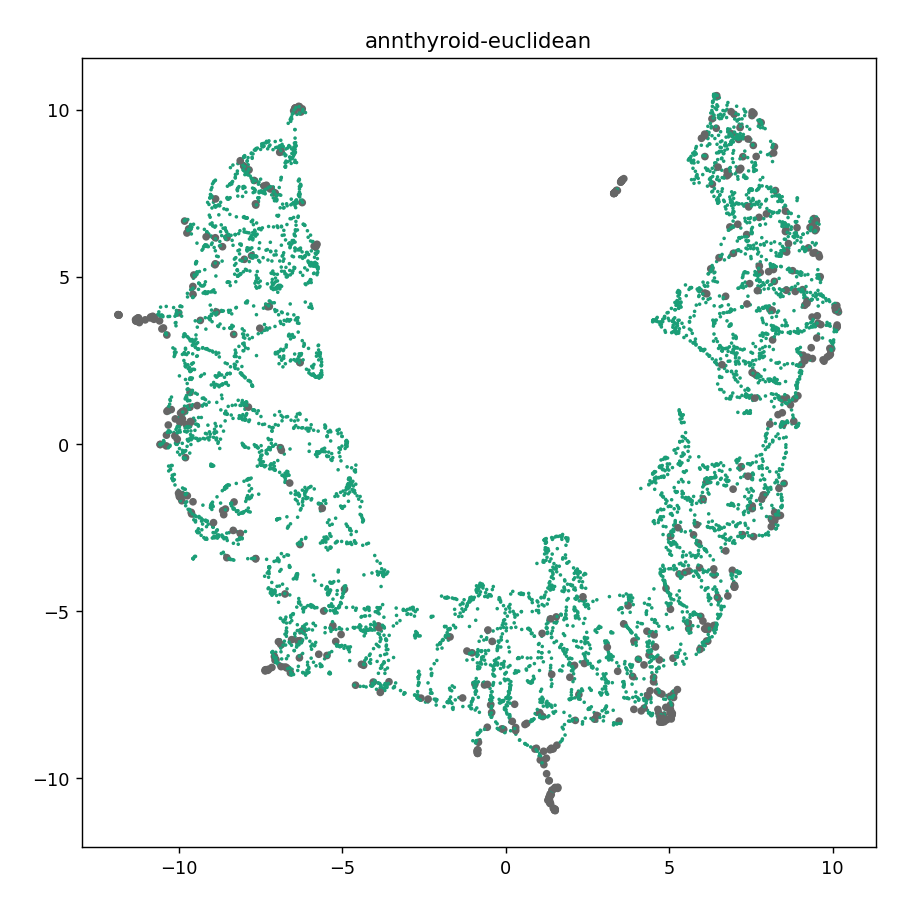
\includegraphics[width=2.5in]{images/umaps/annthyroid-euclidean-umap2d.png}
    \caption{UMAP embedding of Annthyroid data with the Euclidean distance function.}
    \label{fig:discussion:umap-annthyroid-euclidean}
\end{figure}

\subsection{APOGEE-2}
\label{subsec:datasets:apogee-2}

euclidean, cosine, wasserstein-1d

\dots

\subsection{MaNGA}
\label{subsec:datasets:manga}

euclidean, wasserstein-2d

\dots

\subsection{Silva 18S and variants}
\label{subsec:datasets:silva-18s}

hamming, levenshtein

\dots

\subsection{ANN-Benchmarks suite}
\label{subsec:datasets:ann-benchmarks-suite}

deep1b: cosine

fashion-mnist: euclidean

gist: euclidean

glove: cosine

kosarak: jaccard

mnist: euclidean

nytimes: cosine

sift: euclidean

last.fm: cosine

\dots

    \section{Results}
\label{sec:results}

Write about results \dots

Specs of Ark, and maybe M1 MacBook Air and Dell XPS.

Provide link to source code on GitHub.

For each pair $(X, f)$ and a small selection of depths, measure:
\begin{enumerate}[1.]
    \item linear search vs accelerated search:
    \begin{enumerate}[i.]
        \item runtime performance,
        \item speedup factor, and
        \item number of distance comparisons.
    \end{enumerate}
    \item Compression CAKES + zlib vs just zlib, also substitute other libraries for zlib:
    \begin{enumerate}[i.]
        \item just the encoding vs the full dataset,
        \item encoding + serialization, and
        \item encoding + serialization + zlib.
    \end{enumerate}
    \item Measure time taken for accelerated-search in the compressed space and decompression of the hits with different combinations of serde and codec libraries.
\end{enumerate}

Find the optimal clusters for compression.
Compare linear search vs accelerated search terminated at these optimal clusters.

    \section{Discussion}
\label{sec:discussion}

Discuss results and future work \dots

CLAM-CAKES.
This is most effective when datasets exhibit low metric entropy and low local fractal dimension.

Unlike LSH, this is extensible to any user provided distance function.

Exactness of search and metric vs non-metric.

Is it the case that the optimal clusters for compression are also the optimal clusters for accelerated search?

What kind of trade-offs can we offer for space-savings of compression vs time-savings of accelerated-search in the compressed space?

\subsection{Future Works}
\label{subsec:results:future-works}

GPU-acceleration for the more computationally intensive distance functions like wasserstein.

Live-updates as new points are added to the dataset.
For example, build tree with a subsample of the full data and then add the rest of the instances to simulate live-updates.

More distance functions. For example, Tanimoto Distance using maximal-common-subgraph for molecular structures.

Better methods for constructing minimal encodings, perhaps using domain expertise.


    \section*{Acknowledgments}

    \dots

    \FloatBarrier
    \bibliographystyle{unsrt}  
    \bibliography{references}


\end{document}
